\documentclass[conference]{IEEEtran}
\usepackage{cite}
\usepackage{amsmath,amssymb,amsfonts}
\usepackage{algorithmic}
\usepackage{graphicx}
\usepackage{siunitx}
\usepackage{textcomp}
\usepackage{xcolor}
\usepackage{multirow}
\usepackage{url}
\usepackage{epstopdf}
\usepackage{placeins}
\usepackage[inkscapeformat=png]{svg}
\usepackage[font=small,labelfont=bf]{caption}

\epstopdfDeclareGraphicsRule{.gif}{png}{.png}{convert gif:#1 png:\OutputFile}
\AppendGraphicsExtensions{.gif}

\begin{document}

\title{Teaching a Convolutional Neural Network to perform transformations}

\author{\IEEEauthorblockN{Mihai Bojescu}
\IEEEauthorblockA{\textit{Master in Artificial Intelligence and Optimisation} \\
\textit{Faculty of Computer Science of University ``Alexandru Ioan Cuza'' of Iași}\\
Iași, Romania \\
bojescu.mihai@gmail.com}
}

\maketitle


\begin{abstract}
This document contains details on how to make a Convolutional Neural Network learn to perform certain transformations, its
architecture, the loss function used when training, the results of the model and comparisons between the results of the model
and the actual transformations.
\end{abstract}

\begin{IEEEkeywords}
neural network, convolution, convolutional neural network, nn, cnn, transformation, images, loss function
\end{IEEEkeywords}


\section{Introduction}
Convolutional neural networks can be trained to perform a lot of image-related tasks, most of them falling into two categories:
regression and classification. This document details how a Convolutional Neural Network was ``taught'' how to perform
the following transformations:

\begin{enumerate}
    \item resize the image from $32 \times 32$ pixels to $28 \times 28$ pixels
    \item grayscale the image
    \item horizontal flip the image
    \item vertical flip the image
\end{enumerate}

The following chapter will detail the architecture of the network and its parameters.

\section{Architecture}
The model in this project is composed from the following layers:

\begin{enumerate}
    \item 2 Convolutional layers
    \item 1 Max pooling 2D layer
    \item 2 Fully-connected layers
\end{enumerate}

Each convolutional layer goes through a MaxPooling2D pooling function. The result of these layers go through the fully-connected
layers. The model was constructed to be relatively lightweight such that it can perform the ``taught'' transformations with
haste, and relatively accurate such that its outputs can be more beliveable.

\section{Layer parameters}
The aforementioned layers used in the model described in this document use the following parameters:

\begin{enumerate}
    \item $1^{st}$ Convolutional layer:
    \begin{itemize}
        \item Input channels: $3$
        \item Output channels: $32$
        \item Kernel size: $3$
    \end{itemize}
    \item $2^{nd}$ Convolutional layer:
    \begin{itemize}
        \item Input channels: $32$
        \item Output channels: $64$
        \item Kernel size: $3$
    \end{itemize}
    \item The Max pooling 2D layer:
    \begin{itemize}
        \item Kernel size: $2$
        \item Stride: $2$
        \item Padding: $0$
    \end{itemize}
    \item $1^{st}$ Fully-connected layer:
    \begin{itemize}
        \item Size of $(64 * 36) \times 512$
    \end{itemize}
    \item $2^{nd}$ Fully-connected layer:
    \begin{itemize}
        \item Size of $512 \times (28 * 28)$
    \end{itemize}
\end{enumerate}

\section{The loss function}
For the training of the model, the ``MSE'' loss was picked for the following reasons:

\begin{enumerate}
    \item It penalizes larger error more heavily than smaller ones due to the squaring operation. As this model performs
    image regression, large errors are more easily seen, thus they should be minimised the most.
    \item It provides easy-to-understand results. The calculations can be performed on paper in an easier way compared to
    a sigmoid function.
    \item It is a commonly used loss function for various regression tasks, including image regression.
\end{enumerate}

The chosen loss function has a few downsides though:

\begin{enumerate}
    \item It is sensitive to outliers (example: intensity 0 pixels, intensity 255 pixels), which will disproportionately
    infuence the loss.
    \item It does not produce accurate results pixel-wise, thus the images will look blurry.
\end{enumerate}

\section{Early stopping}
In this project, a new concept was introduced to the model trainer, which is ``early stopping''. Early stopping is a way to
decrease the chance of model overfitting by stopping the training process once the model did not minimise the loss for a
certain amount of epochs, named ``delay'' or ``patience''.

For the current iteration of the model trainer, a ``patience'' quota of 5 epochs was chosen. This hyperparameter was chosen
from some observations of the model's behaviour, which:

\begin{itemize}
    \item stopped \textit{too early} when given $patience < 5$
    \item overfitted \textit{too much} when given $patience > 5$, as it trained for all the epochs
\end{itemize}

\section{Training}
When training, the losses trended downards, bottoming at 50 epochs:

\begin{center}
    \begin{minipage}{0.75\linewidth}
        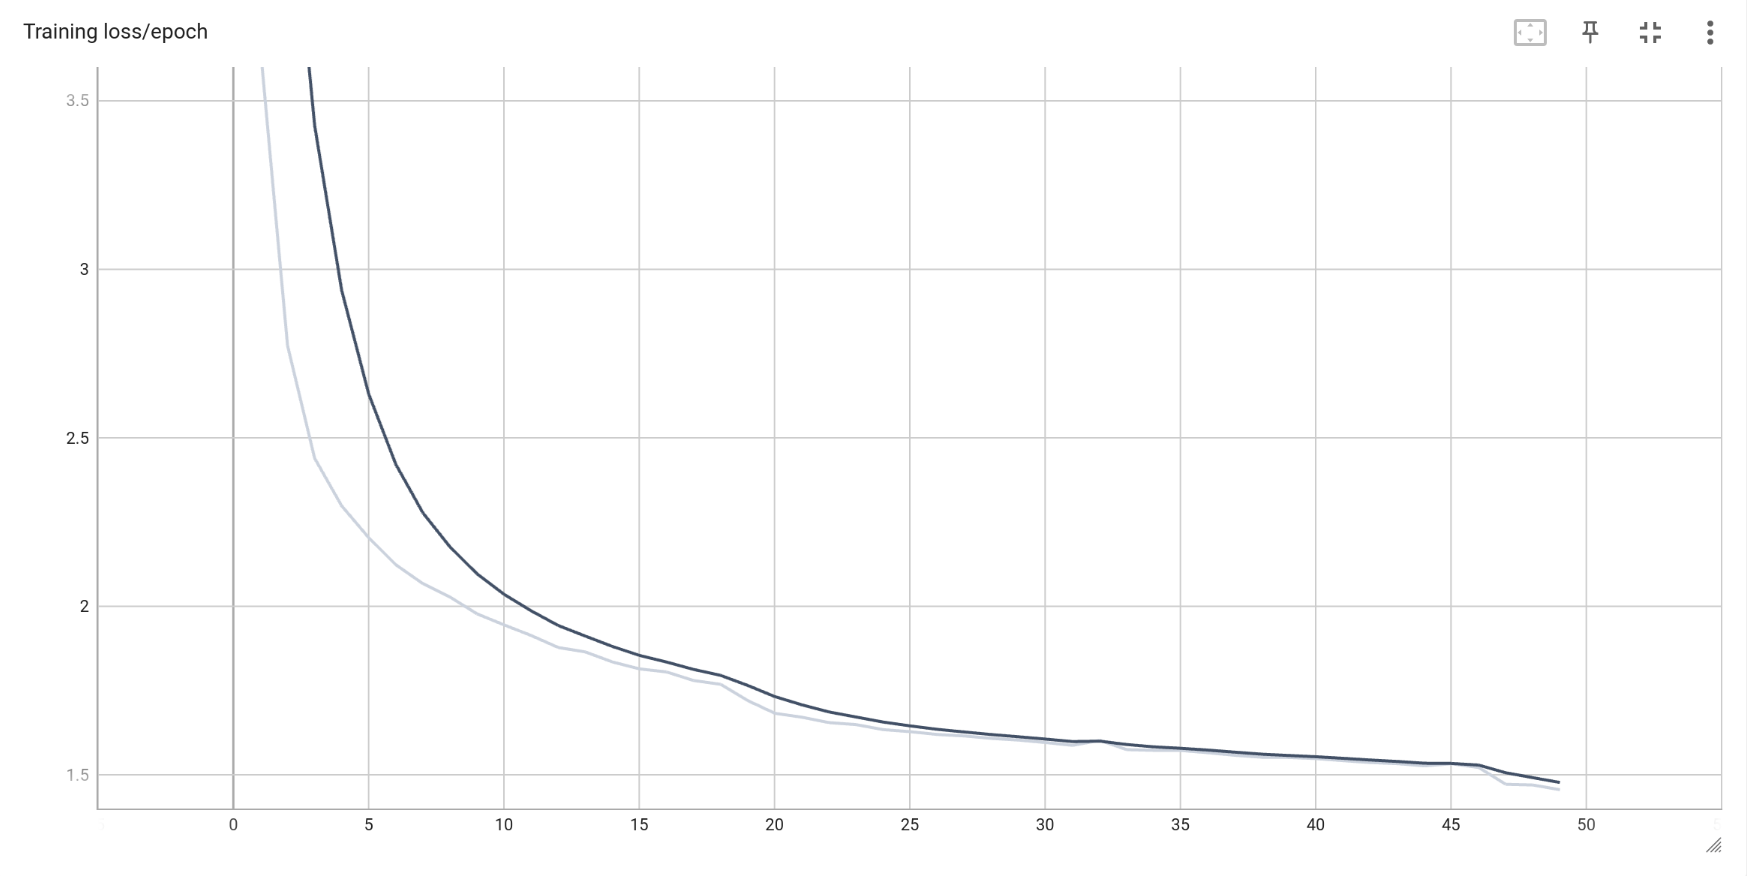
\includegraphics[width=\linewidth]{images/training_loss_graph.png}
        \captionof{figure}{Training loss graph}
    \end{minipage}
\end{center}
\begin{center}
    \begin{minipage}{0.75\linewidth}
        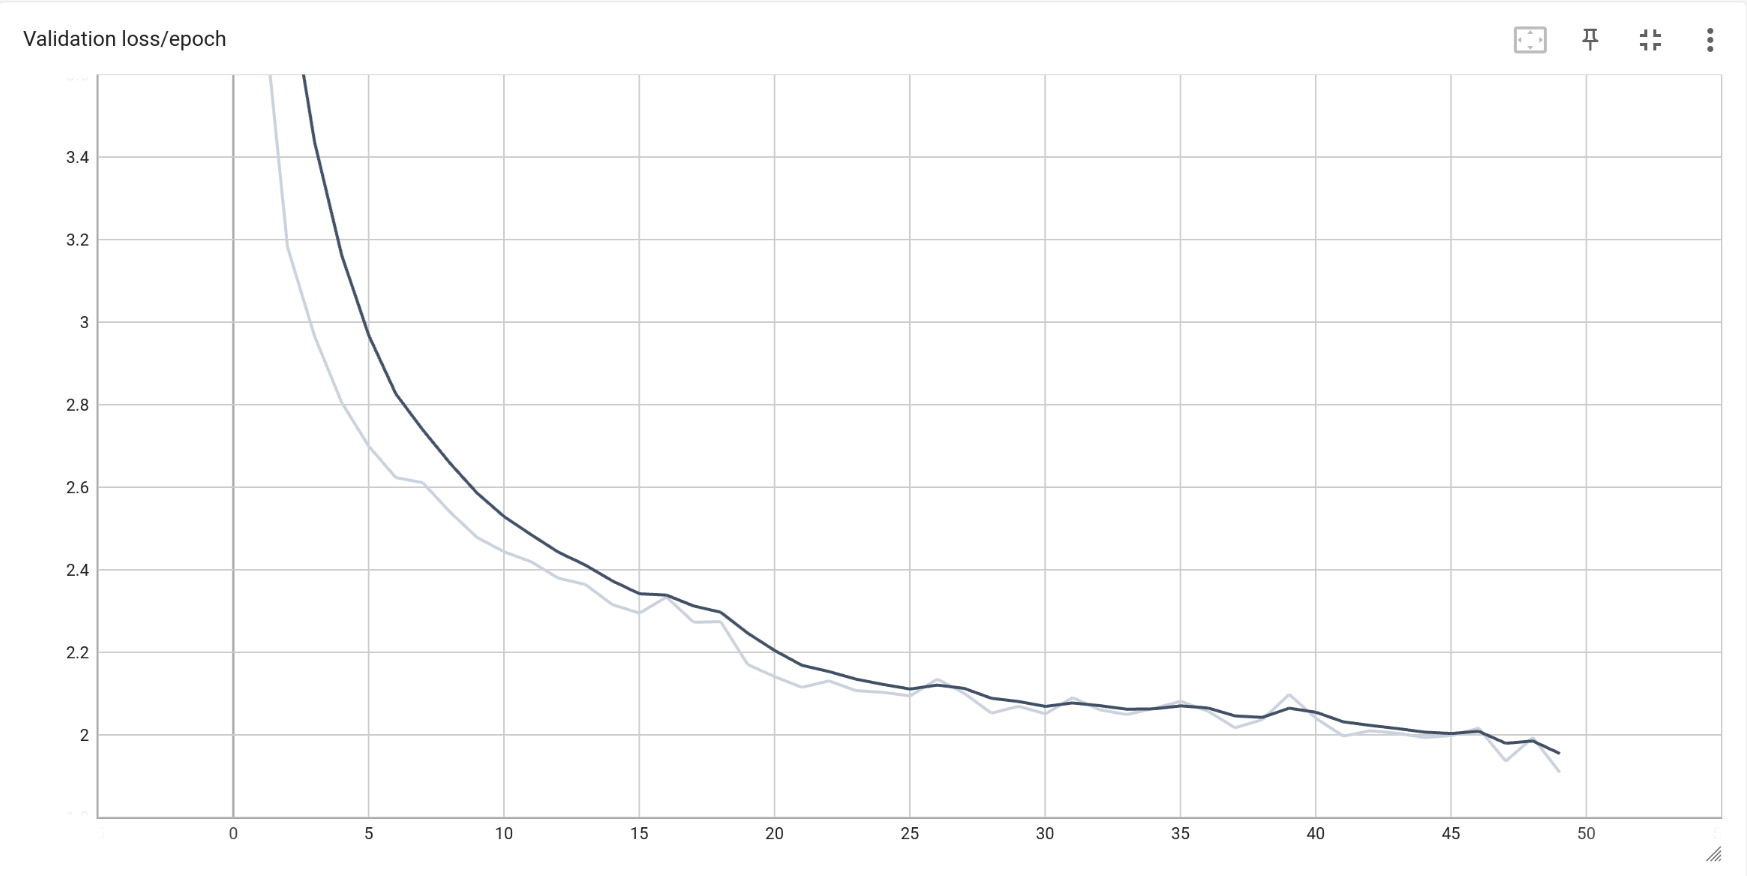
\includegraphics[width=\linewidth]{images/validation_loss_graph.png}
        \captionof{figure}{Validation loss graph}
    \end{minipage}
\end{center}

While the accuracy trended upwards in a constant manner, plateaing at about 50 epochs:

\begin{center}
    \begin{minipage}{0.75\linewidth}
        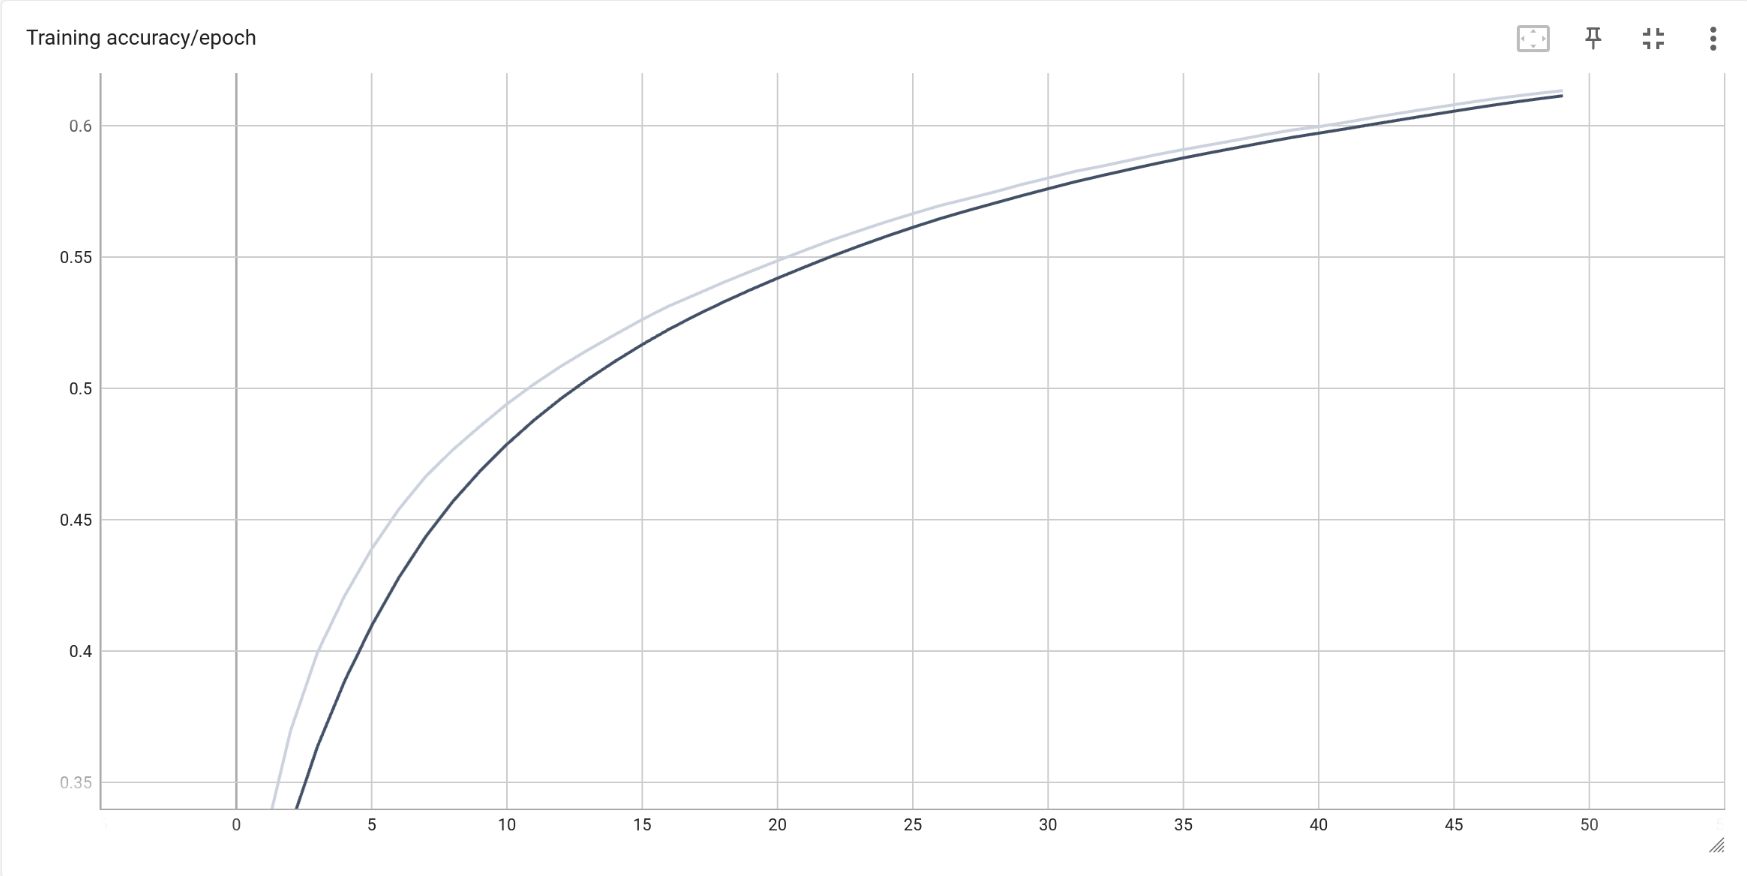
\includegraphics[width=\linewidth]{images/training_accuracy_graph.png}
        \captionof{figure}{Training accuracy graph}
    \end{minipage}
\end{center}
\begin{center}
    \begin{minipage}{0.75\linewidth}
        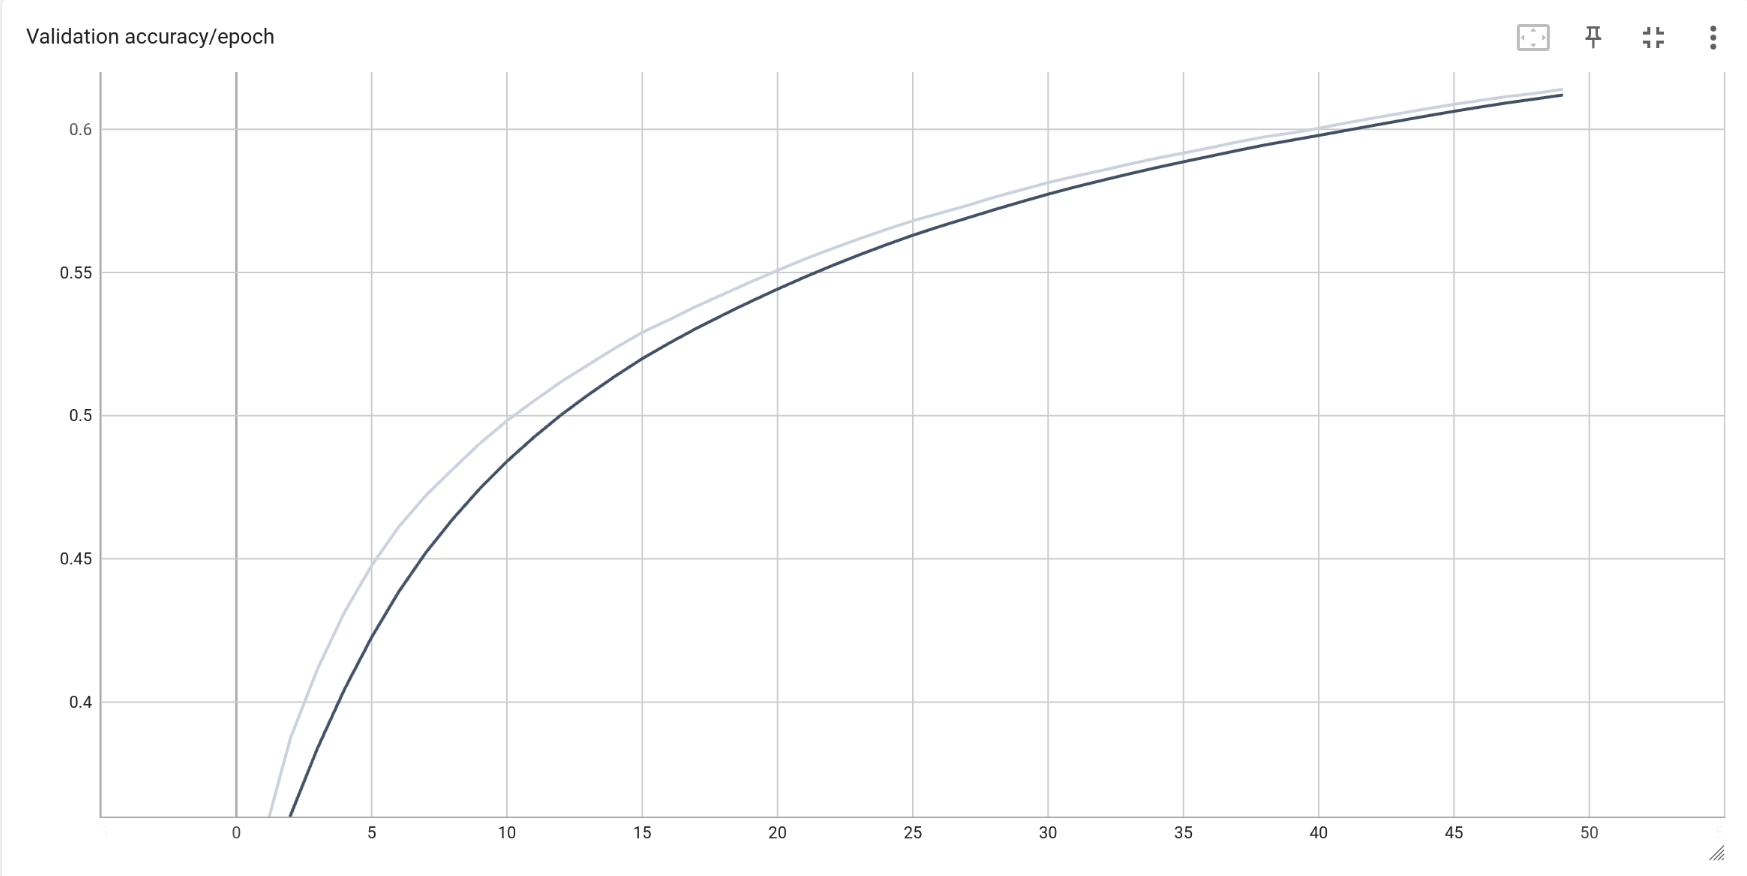
\includegraphics[width=\linewidth]{images/validation_accuracy_graph.png}
        \captionof{figure}{Validation accuracy graph}
    \end{minipage}
\end{center}

\section{Results}

\subsection{Outputs and comparison with the ground truths}
The model can produce fairly convincing pictures, especially when the inputs present the following traits:

\begin{enumerate}
    \item A consistent background
    \item A high contrast
    \item Many straight edges
\end{enumerate}

The results are not perfect though, as they are really blurry and present some distinct artifacts. The model faces problems
especially with:

\begin{enumerate}
    \item Pets against backgrounds
    \item Low contrast pictures
\end{enumerate}

Some results, compared to the ground truths for the model would be:

\begin{center}
    \begin{minipage}{0.75\linewidth}
        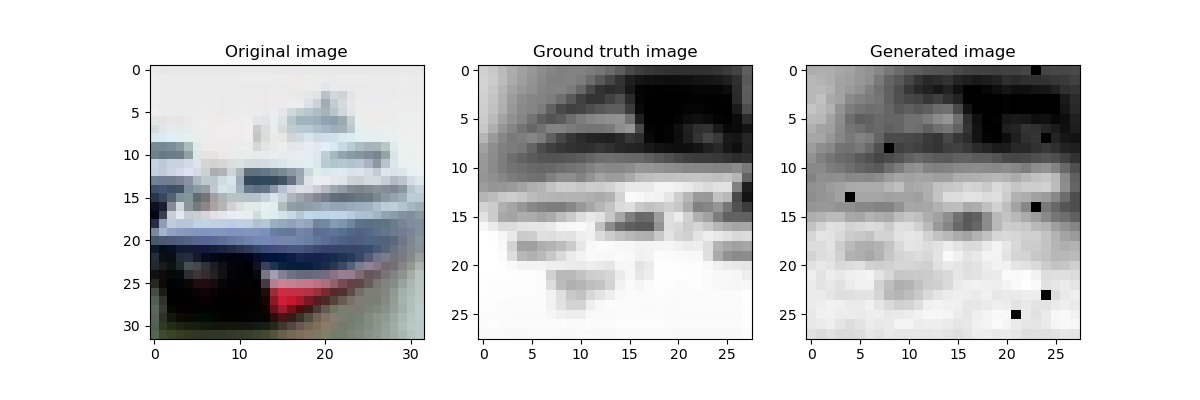
\includegraphics[width=\linewidth]{images/output_1.png}
        \captionof{figure}{A docked boat}
    \end{minipage}
\end{center}
\begin{center}
    \begin{minipage}{0.75\linewidth}
        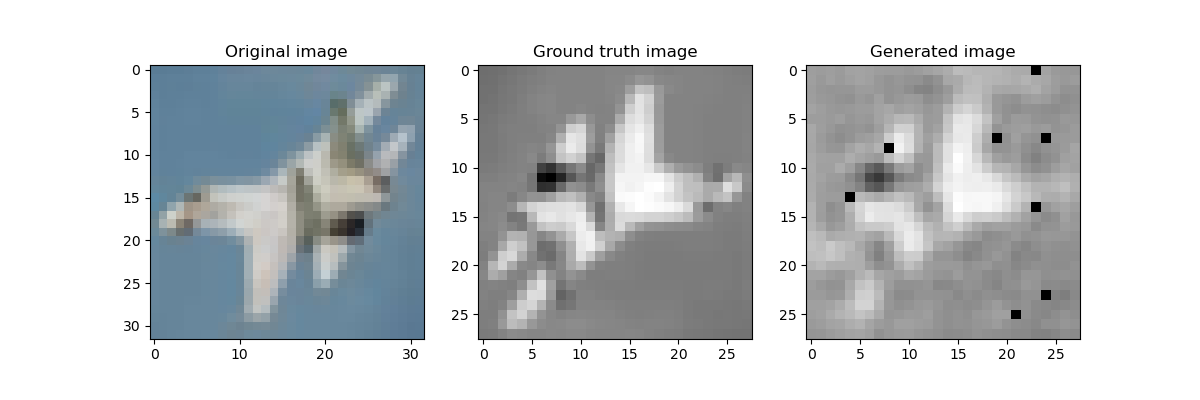
\includegraphics[width=\linewidth]{images/output_10.png}
        \captionof{figure}{A plane in the sky}
    \end{minipage}
\end{center}
\begin{center}
    \begin{minipage}{0.75\linewidth}
        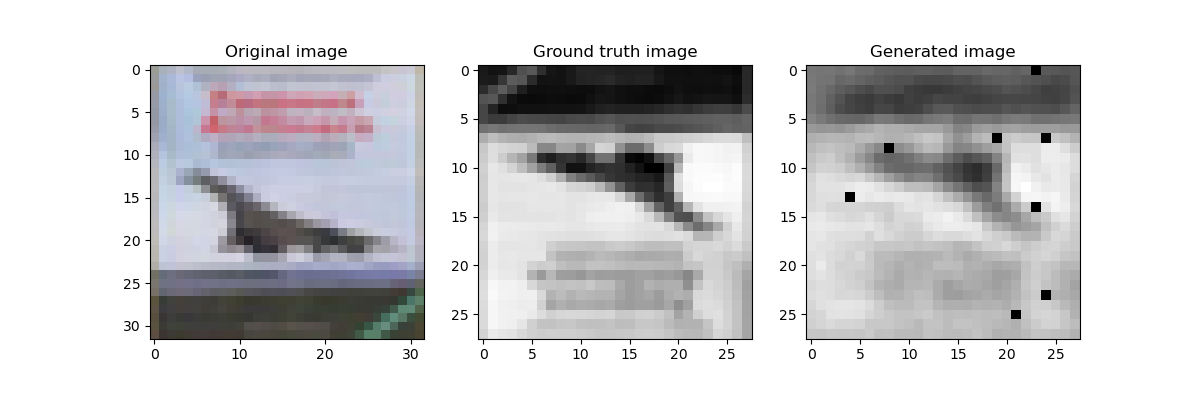
\includegraphics[width=\linewidth]{images/output_3.png}
        \captionof{figure}{A bird in the sky}
    \end{minipage}
\end{center}
\begin{center}
    \begin{minipage}{0.75\linewidth}
        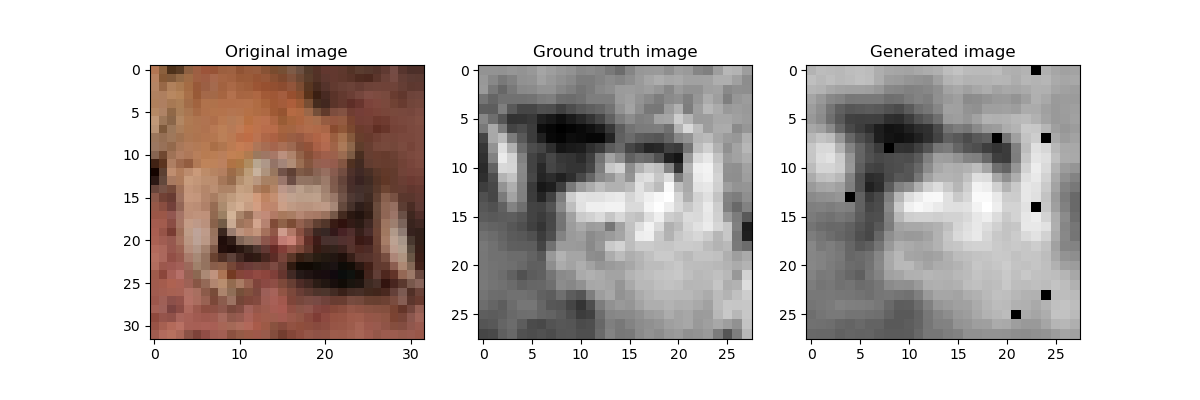
\includegraphics[width=\linewidth]{images/output_5.png}
        \captionof{figure}{A frog on rocks}
    \end{minipage}
\end{center}
\begin{center}
    \begin{minipage}{0.75\linewidth}
        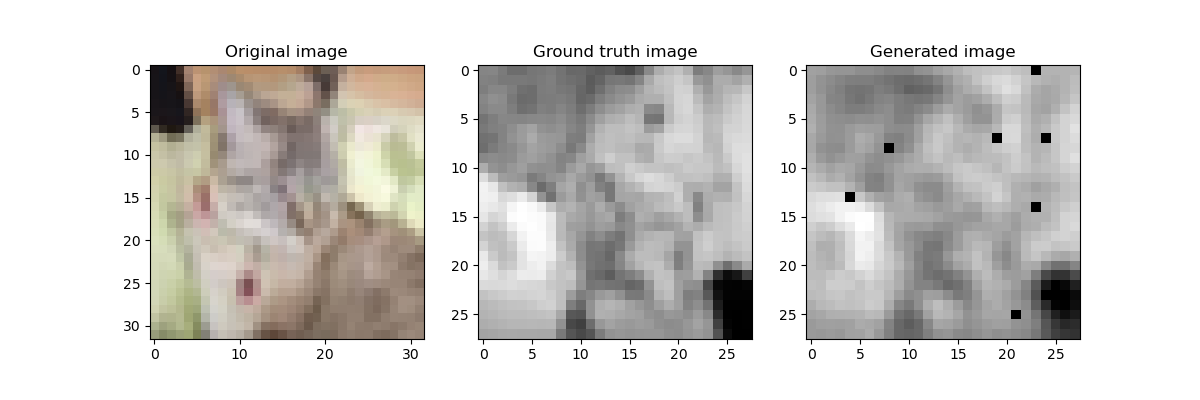
\includegraphics[width=\linewidth]{images/output_8.png}
        \captionof{figure}{A cat against a background}
    \end{minipage}
\end{center}

\subsection{Timings}
During the experimentation phase, the following trends could be seen for the previously outlined model:

\begin{enumerate}
    \item The model performed the actions slower than the transformations on the CPU
    \item The model performed the actions faster than the transformations on the GPU
\end{enumerate}

The observations were performed when running the model on the following configurations:

\begin{enumerate}
    \item CPU runs: 1 x Intel Core i7 1260p
    \item GPU runs: 1 x Nvidia RTX A5000
\end{enumerate}

\textbf{NOTE}: The CPU and GPU runs used different CPUs, as the GPU was rented from a cloud provider. This is the reason
for the rather big differences in the timings for the transformations.

An abstract of the results would be the following:

\begin{center}
    \begin{tabular}{|l|l|l|}
    \hline
        Run & Timing for transformations & Timing for model \\ \hline
        1 & 1.1458s & 1.2898s \\ \hline
        2 & 0.9764s & 1.2944s \\ \hline
        3 & 0.9786s & 1.1745s \\ \hline
        4 & 0.9837s & 1.2515s \\ \hline
        5 & 0.9729s & 1.3458s \\ \hline
    \end{tabular}
    \captionof{figure}{Timing results for running the trained model on the CPU}
\end{center}

\begin{center}
    \begin{tabular}{|l|l|l|}
        \hline
        Run & Timing for transformations & Timing for model \\ \hline
        1 & 1.5567s & 0.4800s \\ \hline
        2 & 1.5094s & 0.4755s \\ \hline
        3 & 1.5700s & 0.4562s \\ \hline
        4 & 1.5671s & 0.5263s \\ \hline
        5 & 1.5739s & 0.4927s \\ \hline
    \end{tabular}
    \captionof{figure}{Timing results for running the trained model on the GPU}
\end{center}

The experiments above back up the trends observed for the model.

\section{Conclusions}
While a simple fully-connected neural network stuggles with beliveable results when performing regression tasks (such as Lab04),
a convolutional neural network can perform these actions better, abeit with a higher computational cost. While being stochastic
in nature, Neural networks can also be ``taught'' to perform actions that deterministic algorithms do with great amounts of
accuracy.

\end{document}
